% Options for packages loaded elsewhere
% Options for packages loaded elsewhere
\PassOptionsToPackage{unicode}{hyperref}
\PassOptionsToPackage{hyphens}{url}
%
\documentclass[
  ignorenonframetext,
  aspectratio=169,
  russian,
  aspectratio=169]{beamer}
\newif\ifbibliography
\usepackage{pgfpages}
\setbeamertemplate{caption}[numbered]
\setbeamertemplate{caption label separator}{: }
\setbeamercolor{caption name}{fg=normal text.fg}
\beamertemplatenavigationsymbolshorizontal
% remove section numbering
\setbeamertemplate{part page}{
  \centering
  \begin{beamercolorbox}[sep=16pt,center]{part title}
    \usebeamerfont{part title}\insertpart\par
  \end{beamercolorbox}
}
\setbeamertemplate{section page}{
  \centering
  \begin{beamercolorbox}[sep=12pt,center]{section title}
    \usebeamerfont{section title}\insertsection\par
  \end{beamercolorbox}
}
\setbeamertemplate{subsection page}{
  \centering
  \begin{beamercolorbox}[sep=8pt,center]{subsection title}
    \usebeamerfont{subsection title}\insertsubsection\par
  \end{beamercolorbox}
}
% Prevent slide breaks in the middle of a paragraph
\widowpenalties 1 10000
\raggedbottom
\AtBeginPart{
  \frame{\partpage}
}
\AtBeginSection{
  \ifbibliography
  \else
    \frame{\sectionpage}
  \fi
}
\AtBeginSubsection{
  \frame{\subsectionpage}
}
\usepackage{iftex}
\ifPDFTeX
  \usepackage[T1]{fontenc}
  \usepackage[utf8]{inputenc}
  \usepackage{textcomp} % provide euro and other symbols
\else % if luatex or xetex
  \usepackage{unicode-math} % this also loads fontspec
  \defaultfontfeatures{Scale=MatchLowercase}
  \defaultfontfeatures[\rmfamily]{Ligatures=TeX,Scale=1}
\fi
\usepackage{lmodern}

\usefonttheme{serif} % use mainfont rather than sansfont for slide text
\ifPDFTeX\else
  % xetex/luatex font selection
  \setmainfont[]{DejaVu Serif}
  \setsansfont[]{DejaVu Sans}
  \setmonofont[]{DejaVu Sans Mono}
\fi
% Use upquote if available, for straight quotes in verbatim environments
\IfFileExists{upquote.sty}{\usepackage{upquote}}{}
\IfFileExists{microtype.sty}{% use microtype if available
  \usepackage[]{microtype}
  \UseMicrotypeSet[protrusion]{basicmath} % disable protrusion for tt fonts
}{}

\usepackage{color}
\usepackage{fancyvrb}
\newcommand{\VerbBar}{|}
\newcommand{\VERB}{\Verb[commandchars=\\\{\}]}
\DefineVerbatimEnvironment{Highlighting}{Verbatim}{commandchars=\\\{\}}
% Add ',fontsize=\small' for more characters per line
\usepackage{framed}
\definecolor{shadecolor}{RGB}{241,243,245}
\newenvironment{Shaded}{\begin{snugshade}}{\end{snugshade}}
\newcommand{\AlertTok}[1]{\textcolor[rgb]{0.68,0.00,0.00}{#1}}
\newcommand{\AnnotationTok}[1]{\textcolor[rgb]{0.37,0.37,0.37}{#1}}
\newcommand{\AttributeTok}[1]{\textcolor[rgb]{0.40,0.45,0.13}{#1}}
\newcommand{\BaseNTok}[1]{\textcolor[rgb]{0.68,0.00,0.00}{#1}}
\newcommand{\BuiltInTok}[1]{\textcolor[rgb]{0.00,0.23,0.31}{#1}}
\newcommand{\CharTok}[1]{\textcolor[rgb]{0.13,0.47,0.30}{#1}}
\newcommand{\CommentTok}[1]{\textcolor[rgb]{0.37,0.37,0.37}{#1}}
\newcommand{\CommentVarTok}[1]{\textcolor[rgb]{0.37,0.37,0.37}{\textit{#1}}}
\newcommand{\ConstantTok}[1]{\textcolor[rgb]{0.56,0.35,0.01}{#1}}
\newcommand{\ControlFlowTok}[1]{\textcolor[rgb]{0.00,0.23,0.31}{\textbf{#1}}}
\newcommand{\DataTypeTok}[1]{\textcolor[rgb]{0.68,0.00,0.00}{#1}}
\newcommand{\DecValTok}[1]{\textcolor[rgb]{0.68,0.00,0.00}{#1}}
\newcommand{\DocumentationTok}[1]{\textcolor[rgb]{0.37,0.37,0.37}{\textit{#1}}}
\newcommand{\ErrorTok}[1]{\textcolor[rgb]{0.68,0.00,0.00}{#1}}
\newcommand{\ExtensionTok}[1]{\textcolor[rgb]{0.00,0.23,0.31}{#1}}
\newcommand{\FloatTok}[1]{\textcolor[rgb]{0.68,0.00,0.00}{#1}}
\newcommand{\FunctionTok}[1]{\textcolor[rgb]{0.28,0.35,0.67}{#1}}
\newcommand{\ImportTok}[1]{\textcolor[rgb]{0.00,0.46,0.62}{#1}}
\newcommand{\InformationTok}[1]{\textcolor[rgb]{0.37,0.37,0.37}{#1}}
\newcommand{\KeywordTok}[1]{\textcolor[rgb]{0.00,0.23,0.31}{\textbf{#1}}}
\newcommand{\NormalTok}[1]{\textcolor[rgb]{0.00,0.23,0.31}{#1}}
\newcommand{\OperatorTok}[1]{\textcolor[rgb]{0.37,0.37,0.37}{#1}}
\newcommand{\OtherTok}[1]{\textcolor[rgb]{0.00,0.23,0.31}{#1}}
\newcommand{\PreprocessorTok}[1]{\textcolor[rgb]{0.68,0.00,0.00}{#1}}
\newcommand{\RegionMarkerTok}[1]{\textcolor[rgb]{0.00,0.23,0.31}{#1}}
\newcommand{\SpecialCharTok}[1]{\textcolor[rgb]{0.37,0.37,0.37}{#1}}
\newcommand{\SpecialStringTok}[1]{\textcolor[rgb]{0.13,0.47,0.30}{#1}}
\newcommand{\StringTok}[1]{\textcolor[rgb]{0.13,0.47,0.30}{#1}}
\newcommand{\VariableTok}[1]{\textcolor[rgb]{0.07,0.07,0.07}{#1}}
\newcommand{\VerbatimStringTok}[1]{\textcolor[rgb]{0.13,0.47,0.30}{#1}}
\newcommand{\WarningTok}[1]{\textcolor[rgb]{0.37,0.37,0.37}{\textit{#1}}}

\usepackage{longtable,booktabs,array}
\newcounter{none} % for unnumbered tables
\usepackage{calc} % for calculating minipage widths
\usepackage{caption}
% Make caption package work with longtable
\makeatletter
\def\fnum@table{\tablename~\thetable}
\makeatother
\usepackage{graphicx}
\makeatletter
\newsavebox\pandoc@box
\newcommand*\pandocbounded[1]{% scales image to fit in text height/width
  \sbox\pandoc@box{#1}%
  \Gscale@div\@tempa{\textheight}{\dimexpr\ht\pandoc@box+\dp\pandoc@box\relax}%
  \Gscale@div\@tempb{\linewidth}{\wd\pandoc@box}%
  \ifdim\@tempb\p@<\@tempa\p@\let\@tempa\@tempb\fi% select the smaller of both
  \ifdim\@tempa\p@<\p@\scalebox{\@tempa}{\usebox\pandoc@box}%
  \else\usebox{\pandoc@box}%
  \fi%
}
% Set default figure placement to htbp
\def\fps@figure{htbp}
\makeatother



\ifLuaTeX
\usepackage[bidi=basic,shorthands=off,provide=*]{babel}
\else
\usepackage[bidi=default,shorthands=off,provide=*]{babel}
\fi
\ifPDFTeX
\else
\babelfont{rm}[]{DejaVu Serif}
\fi
\ifLuaTeX
  \usepackage{selnolig} % disable illegal ligatures
\fi


\setlength{\emergencystretch}{3em} % prevent overfull lines

\providecommand{\tightlist}{%
  \setlength{\itemsep}{0pt}\setlength{\parskip}{0pt}}



 

\usepackage[]{csquotes}

\IfFileExists{plex-otf.sty}{
  %% Full TeXlive
  % \usepackage[%
  %   % math,
  %   RM={Scale=0.94},SS={Scale=0.94},SScon={Scale=0.94},TT={Scale=MatchLowercase,FakeStretch=0.9},DefaultFeatures={Ligatures=Common}
  % ]{plex-otf}
}{
  %% TinyTeX
  \usepackage{libertine}
}

%%% Load theme
% https://deic.uab.cat/~iblanes/beamer_gallery/
\IfFileExists{beamerthemegotham.sty}{
  %% Full TeXlive
  \usetheme{gotham}
  \gothamset{
    numbering=totalpagenumber,
    parttocframe default=off,
    sectiontocframe default=off,
    subsectiontocframe default=off,
  }
}{
  %% TinyTeX
  \usetheme{Madrid}
}
\makeatletter
\@ifpackageloaded{caption}{}{\usepackage{caption}}
\AtBeginDocument{%
\ifdefined\contentsname
  \renewcommand*\contentsname{Содержание}
\else
  \newcommand\contentsname{Содержание}
\fi
\ifdefined\listfigurename
  \renewcommand*\listfigurename{Список иллюстраций}
\else
  \newcommand\listfigurename{Список иллюстраций}
\fi
\ifdefined\listtablename
  \renewcommand*\listtablename{Список таблиц}
\else
  \newcommand\listtablename{Список таблиц}
\fi
\ifdefined\figurename
  \renewcommand*\figurename{Рисунок}
\else
  \newcommand\figurename{Рисунок}
\fi
\ifdefined\tablename
  \renewcommand*\tablename{Таблица}
\else
  \newcommand\tablename{Таблица}
\fi
}
\@ifpackageloaded{float}{}{\usepackage{float}}
\floatstyle{ruled}
\@ifundefined{c@chapter}{\newfloat{codelisting}{h}{lop}}{\newfloat{codelisting}{h}{lop}[chapter]}
\floatname{codelisting}{Список}
\newcommand*\listoflistings{\listof{codelisting}{Листинги}}
\makeatother
\makeatletter
\makeatother
\makeatletter
\@ifpackageloaded{caption}{}{\usepackage{caption}}
\@ifpackageloaded{subcaption}{}{\usepackage{subcaption}}
\makeatother

\usepackage{bookmark}
\IfFileExists{xurl.sty}{\usepackage{xurl}}{} % add URL line breaks if available
\urlstyle{same}
\hypersetup{
  pdftitle={Выполнение лабораторной работы №7},
  pdfauthor={Карпухин Клим},
  pdflang={ru-RU},
  hidelinks,
  pdfcreator={LaTeX via pandoc}}


\title{\texorpdfstring{Выполнение лабораторной работы
№7}{Выполнение лабораторной работы №7}}
\subtitle{\texorpdfstring{Анализ файловой системы Linux. Команды для
работы с файлами и
каталогами.}{Анализ файловой системы Linux. Команды для работы с файлами и каталогами.}}
\author{Карпухин Клим}
\date{2026-03-28}

\begin{document}
\frame{\titlepage}


\section{Содержание}\label{ux441ux43eux434ux435ux440ux436ux430ux43dux438ux435}

\begin{frame}{Содержание}
\begin{enumerate}[<+->]
\tightlist
\item
  Информация о докладчике
\item
  Актуальность и цель работы
\item
  Теоретические основы
\item
  Ход работы: работа с Midnight Commander
\item
  Ход работы: команды для работы с файлами
\item
  Управление правами доступа
\item
  Системные команды (mount, fsck, mkfs, kill)
\item
  Контрольные вопросы
\item
  Выводы
\end{enumerate}
\end{frame}

\section{Информация}\label{ux438ux43dux444ux43eux440ux43cux430ux446ux438ux44f}

\begin{frame}{Докладчик}
\protect\phantomsection\label{ux434ux43eux43aux43bux430ux434ux447ux438ux43a}
\begin{columns}[c]
\begin{column}{0.65\linewidth}
\begin{itemize}[<+->]
\tightlist
\item
  \textbf{Карпухин Клим}
\item
  Российский университет дружбы народов
\item
  Email:
  \href{mailto:1032255580@rudn.ru}{\nolinkurl{1032255580@rudn.ru}}
\item
  Роль: студент (лабораторная работа по ОС)
\end{itemize}
\end{column}

\begin{column}{0.35\linewidth}

\includegraphics[width=0.9\linewidth,height=\textheight,keepaspectratio]{./image/dokladchik.png}
\end{column}
\end{columns}
\end{frame}

\section{Актуальность и цель
работы}\label{ux430ux43aux442ux443ux430ux43bux44cux43dux43eux441ux442ux44c-ux438-ux446ux435ux43bux44c-ux440ux430ux431ux43eux442ux44b}

\begin{frame}[fragile]{Актуальность}
\protect\phantomsection\label{ux430ux43aux442ux443ux430ux43bux44cux43dux43eux441ux442ux44c}
\begin{itemize}[<+->]
\tightlist
\item
  Файловая система Linux имеет строгую иерархическую структуру, знание
  которой необходимо для эффективной работы.
\item
  Команды для работы с файлами (\texttt{cp}, \texttt{mv},
  \texttt{chmod}) являются основой администрирования и повседневной
  деятельности.
\item
  Midnight Commander (mc) значительно ускоряет работу с файловой
  системой в терминале.
\item
  Понимание прав доступа критически важно для обеспечения безопасности
  системы.
\end{itemize}
\end{frame}

\begin{frame}{Цель работы}
\protect\phantomsection\label{ux446ux435ux43bux44c-ux440ux430ux431ux43eux442ux44b}
Ознакомление с файловой системой Linux, её структурой, именами и
содержанием каталогов. Приобретение практических навыков по применению
команд для работы с файлами и каталогами, по управлению процессами, по
проверке использования диска и обслуживанию файловой системы.
\end{frame}

\section{Теоретические
основы}\label{ux442ux435ux43eux440ux435ux442ux438ux447ux435ux441ux43aux438ux435-ux43eux441ux43dux43eux432ux44b}

\begin{frame}[fragile]{Основные команды}
\protect\phantomsection\label{ux43eux441ux43dux43eux432ux43dux44bux435-ux43aux43eux43cux430ux43dux434ux44b}
{\def\LTcaptype{none} % do not increment counter
\begin{longtable}[]{@{}ll@{}}
\toprule\noalign{}
Команда & Назначение \\
\midrule\noalign{}
\endhead
\texttt{touch} & Создание пустого файла / обновление метки времени \\
\texttt{cat} / \texttt{less} / \texttt{head} / \texttt{tail} & Просмотр
содержимого файлов \\
\texttt{cp} & Копирование файлов и каталогов \\
\texttt{mv} & Перемещение / переименование объектов \\
\texttt{chmod} & Изменение прав доступа \\
\texttt{mount} / \texttt{df} & Монтирование и анализ использования
диска \\
\texttt{fsck} / \texttt{mkfs} & Проверка и создание файловых систем \\
\texttt{kill} & Отправка сигналов процессам \\
\bottomrule\noalign{}
\end{longtable}
}
\end{frame}

\section{Ход работы: Midnight
Commander}\label{ux445ux43eux434-ux440ux430ux431ux43eux442ux44b-midnight-commander}

\begin{frame}[fragile]{Запуск и интерфейс mc}
\protect\phantomsection\label{ux437ux430ux43fux443ux441ux43a-ux438-ux438ux43dux442ux435ux440ux444ux435ux439ux441-mc}
\begin{itemize}[<+->]
\tightlist
\item
  Запустил Midnight Commander командой \texttt{mc} в терминале.
\item
  Изучил структуру: две панели, строка меню, командная строка внизу.
\end{itemize}


\includegraphics[width=0.6\linewidth,height=\textheight,keepaspectratio]{./image/1.png}
\end{frame}

\begin{frame}[fragile]{Навигация и функциональные клавиши}
\protect\phantomsection\label{ux43dux430ux432ux438ux433ux430ux446ux438ux44f-ux438-ux444ux443ux43dux43aux446ux438ux43eux43dux430ux43bux44cux43dux44bux435-ux43aux43bux430ux432ux438ux448ux438}
\begin{itemize}[<+->]
\tightlist
\item
  Навигация: клавиши-стрелки, \texttt{Enter} для входа,
  \texttt{Ctrl+PageUp} для выхода.
\item
  Функциональные клавиши:

  \begin{itemize}[<+->]
  \tightlist
  \item
    \texttt{F1} --- справка
  \item
    \texttt{F3} --- просмотр файла
  \item
    \texttt{F4} --- редактирование
  \item
    \texttt{F5} --- копирование
  \item
    \texttt{F6} --- перемещение/переименование
  \item
    \texttt{F7} --- создание каталога
  \item
    \texttt{F8} --- удаление
  \item
    \texttt{F9} --- главное меню
  \item
    \texttt{F10} --- выход
  \end{itemize}
\end{itemize}


\includegraphics[width=0.6\linewidth,height=\textheight,keepaspectratio]{./image/3.png}
\end{frame}

\begin{frame}[fragile]{Работа с панелями}
\protect\phantomsection\label{ux440ux430ux431ux43eux442ux430-ux441-ux43fux430ux43dux435ux43bux44fux43cux438}
\begin{itemize}[<+->]
\tightlist
\item
  Переключение между панелями: \texttt{Tab}
\item
  Установил в левой панели \texttt{/tmp}, в правой --- домашний каталог.
\item
  Изменение формата отображения: \texttt{Левая\ панель} →
  \texttt{Формат\ списка} (стандартный, длинный, с правами доступа).
\end{itemize}


\includegraphics[width=0.6\linewidth,height=\textheight,keepaspectratio]{./image/5.png}
\end{frame}

\begin{frame}[fragile]{Меню «Команда» и поиск}
\protect\phantomsection\label{ux43cux435ux43dux44e-ux43aux43eux43cux430ux43dux434ux430-ux438-ux43fux43eux438ux441ux43a}
\begin{itemize}[<+->]
\tightlist
\item
  Открыл меню \texttt{Команда}: \texttt{Дерево\ каталогов},
  \texttt{Поиск\ файла}, \texttt{Каталоги\ быстрого\ перехода}.
\item
  Нашёл файлы, содержащие слово \texttt{bash}, в каталоге \texttt{/etc}.
\end{itemize}


\includegraphics[width=0.6\linewidth,height=\textheight,keepaspectratio]{./image/16.png}
\end{frame}

\section{Ход работы: просмотр и
редактирование}\label{ux445ux43eux434-ux440ux430ux431ux43eux442ux44b-ux43fux440ux43eux441ux43cux43eux442ux440-ux438-ux440ux435ux434ux430ux43aux442ux438ux440ux43eux432ux430ux43dux438ux435}

\begin{frame}[fragile]{Просмотр и редактирование файлов}
\protect\phantomsection\label{ux43fux440ux43eux441ux43cux43eux442ux440-ux438-ux440ux435ux434ux430ux43aux442ux438ux440ux43eux432ux430ux43dux438ux435-ux444ux430ux439ux43bux43eux432}
\begin{itemize}[<+->]
\tightlist
\item
  \textbf{Просмотр} (\texttt{F3}): открыл текстовый файл для просмотра.
\end{itemize}


\includegraphics[width=0.6\linewidth,height=\textheight,keepaspectratio]{./image/7.png}

\begin{itemize}[<+->]
\tightlist
\item
  \textbf{Редактирование} (\texttt{F4}): открыл файл в редакторе mcedit,
  внёс изменения, сохранил (\texttt{F2}).
\end{itemize}


\includegraphics[width=0.6\linewidth,height=\textheight,keepaspectratio]{./image/8.png}
\end{frame}

\begin{frame}[fragile]{Создание и копирование файлов}
\protect\phantomsection\label{ux441ux43eux437ux434ux430ux43dux438ux435-ux438-ux43aux43eux43fux438ux440ux43eux432ux430ux43dux438ux435-ux444ux430ux439ux43bux43eux432}
\begin{itemize}[<+->]
\tightlist
\item
  Создал новый файл \texttt{test.txt} через редактор (\texttt{F4} при
  несуществующем имени).
\item
  Скопировал файл в \texttt{/tmp} с помощью \texttt{F5}.
\item
  Переименовал копию в \texttt{/tmp} с помощью \texttt{F6}.
\end{itemize}


\includegraphics[width=0.6\linewidth,height=\textheight,keepaspectratio]{./image/10.png}
\end{frame}

\begin{frame}[fragile]{Операции с каталогами}
\protect\phantomsection\label{ux43eux43fux435ux440ux430ux446ux438ux438-ux441-ux43aux430ux442ux430ux43bux43eux433ux430ux43cux438}
\begin{itemize}[<+->]
\tightlist
\item
  Создал каталог \texttt{lab7dir} (\texttt{F7}).
\item
  Скопировал \texttt{test.txt} в созданный каталог.
\item
  Выделение файлов: \texttt{Insert} для выборочного выделения,
  \texttt{+} для выделения по маске (\texttt{*.txt}).
\item
  Удаление выделенных файлов (\texttt{F8}).
\end{itemize}
\end{frame}

\begin{frame}[fragile]{Дерево каталогов и поиск}
\protect\phantomsection\label{ux434ux435ux440ux435ux432ux43e-ux43aux430ux442ux430ux43bux43eux433ux43eux432-ux438-ux43fux43eux438ux441ux43a}
\begin{itemize}[<+->]
\tightlist
\item
  Включил отображение дерева каталогов: \texttt{Панели} →
  \texttt{Дерево\ каталогов}.
\end{itemize}


\includegraphics[width=0.6\linewidth,height=\textheight,keepaspectratio]{./image/15.png}

\begin{itemize}[<+->]
\tightlist
\item
  Использовал встроенный поиск файлов по содержимому (\texttt{Команда} →
  \texttt{Поиск\ файла} или \texttt{Alt+?}).
\end{itemize}
\end{frame}

\begin{frame}[fragile]{Встроенный редактор mcedit}
\protect\phantomsection\label{ux432ux441ux442ux440ux43eux435ux43dux43dux44bux439-ux440ux435ux434ux430ux43aux442ux43eux440-mcedit}
\begin{itemize}[<+->]
\tightlist
\item
  Открыл \texttt{\textasciitilde{}/.bashrc} (\texttt{F4}) и изучил
  возможности редактора:

  \begin{itemize}[<+->]
  \tightlist
  \item
    поиск по тексту (\texttt{F7});
  \item
    замена (\texttt{F4} в режиме поиска);
  \item
    переход к строке (\texttt{Alt+L});
  \item
    включение подсветки синтаксиса.
  \end{itemize}
\item
  Создал файл \texttt{note.txt}, поработал с буфером обмена (\texttt{F5}
  --- копировать, \texttt{F6} --- переместить).
\end{itemize}


\includegraphics[width=0.6\linewidth,height=\textheight,keepaspectratio]{./image/19.png}
\end{frame}

\begin{frame}[fragile]{Меню пользователя и настройки mc}
\protect\phantomsection\label{ux43cux435ux43dux44e-ux43fux43eux43bux44cux437ux43eux432ux430ux442ux435ux43bux44f-ux438-ux43dux430ux441ux442ux440ux43eux439ux43aux438-mc}
\begin{itemize}[<+->]
\tightlist
\item
  \texttt{F2} --- меню пользователя для определения собственных команд.
\item
  \texttt{F9} --- главное меню: \texttt{Левая}, \texttt{Файл},
  \texttt{Команда}, \texttt{Настройки}, \texttt{Правая}.
\item
  В разделе \texttt{Настройки} → \texttt{Внешний\ вид} изменил цветовую
  схему.
\end{itemize}


\includegraphics[width=0.6\linewidth,height=\textheight,keepaspectratio]{./image/23.png}
\end{frame}

\section{Ход работы: задание 2
(псевдонимы)}\label{ux445ux43eux434-ux440ux430ux431ux43eux442ux44b-ux437ux430ux434ux430ux43dux438ux435-2-ux43fux441ux435ux432ux434ux43eux43dux438ux43cux44b}

\begin{frame}[fragile]{Добавление псевдонимов в .bashrc}
\protect\phantomsection\label{ux434ux43eux431ux430ux432ux43bux435ux43dux438ux435-ux43fux441ux435ux432ux434ux43eux43dux438ux43cux43eux432-ux432-.bashrc}
Добавил в файл \texttt{\textasciitilde{}/.bashrc} следующие псевдонимы:

\begin{Shaded}
\begin{Highlighting}[]
\BuiltInTok{alias}\NormalTok{ up=}\StringTok{\textquotesingle{}cd ..\textquotesingle{}}
\BuiltInTok{alias}\NormalTok{ ll=}\StringTok{\textquotesingle{}ls {-}la\textquotesingle{}}
\BuiltInTok{alias}\NormalTok{ h=}\StringTok{\textquotesingle{}history\textquotesingle{}}
\BuiltInTok{alias}\NormalTok{ cls=}\StringTok{\textquotesingle{}clear\textquotesingle{}}
\BuiltInTok{alias}\NormalTok{ grep=}\StringTok{\textquotesingle{}grep {-}{-}color=auto\textquotesingle{}}
\end{Highlighting}
\end{Shaded}

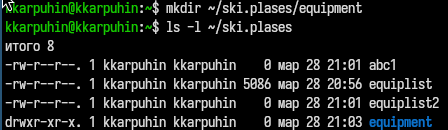
\includegraphics[width=0.6\linewidth,height=\textheight,keepaspectratio]{./image/29.png}
\end{frame}

\begin{frame}[fragile]{Проверка работы псевдонимов}
\protect\phantomsection\label{ux43fux440ux43eux432ux435ux440ux43aux430-ux440ux430ux431ux43eux442ux44b-ux43fux441ux435ux432ux434ux43eux43dux438ux43cux43eux432}
После выполнения \texttt{source\ \textasciitilde{}/.bashrc}:

\begin{itemize}[<+->]
\tightlist
\item
  \texttt{up} --- переход на уровень выше.
\item
  \texttt{ll} --- подробный список файлов.
\item
  \texttt{h} --- история команд.
\item
  \texttt{cls} --- очистка экрана.
\item
  \texttt{grep} --- цветная подсветка вхождений.
\end{itemize}

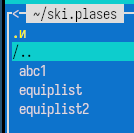
\includegraphics[width=0.6\linewidth,height=\textheight,keepaspectratio]{./image/28.5.png}
\end{frame}

\section{Ход работы: задание 3 и
4}\label{ux445ux43eux434-ux440ux430ux431ux43eux442ux44b-ux437ux430ux434ux430ux43dux438ux435-3-ux438-4}

\begin{frame}[fragile]{Задание 3: команды в командной строке mc}
\protect\phantomsection\label{ux437ux430ux434ux430ux43dux438ux435-3-ux43aux43eux43cux430ux43dux434ux44b-ux432-ux43aux43eux43cux430ux43dux434ux43dux43eux439-ux441ux442ux440ux43eux43aux435-mc}
\begin{itemize}[<+->]
\tightlist
\item
  В командной строке mc выполнил:

  \begin{itemize}[<+->]
  \tightlist
  \item
    \texttt{cat\ /etc/shells} --- список доступных оболочек.
  \item
    \texttt{echo\ \$SHELL} --- текущая оболочка.
  \end{itemize}
\end{itemize}

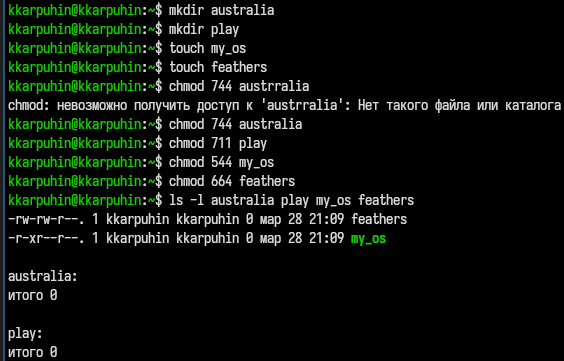
\includegraphics[width=0.6\linewidth,height=\textheight,keepaspectratio]{./image/32.png}
\end{frame}

\begin{frame}[fragile]{Задание 4: упражнения с файлами}
\protect\phantomsection\label{ux437ux430ux434ux430ux43dux438ux435-4-ux443ux43fux440ux430ux436ux43dux435ux43dux438ux44f-ux441-ux444ux430ux439ux43bux430ux43cux438}
\textbf{4.1} Просмотр \texttt{/etc/password} через \texttt{F3}.
\textbf{4.2} Копирование \texttt{\textasciitilde{}/feathers} →
\texttt{\textasciitilde{}/file.old}:

\begin{Shaded}
\begin{Highlighting}[]
\FunctionTok{cp}\NormalTok{ \textasciitilde{}/feathers \textasciitilde{}/file.old}
\end{Highlighting}
\end{Shaded}

\textbf{4.3} Перемещение \texttt{\textasciitilde{}/file.old} →
\texttt{\textasciitilde{}/play}:

\begin{Shaded}
\begin{Highlighting}[]
\FunctionTok{mv}\NormalTok{ \textasciitilde{}/file.old \textasciitilde{}/play}
\end{Highlighting}
\end{Shaded}

\textbf{4.4} Копирование каталога \texttt{\textasciitilde{}/play} →
\texttt{\textasciitilde{}/fun}:

\begin{Shaded}
\begin{Highlighting}[]
\FunctionTok{cp} \AttributeTok{{-}r}\NormalTok{ \textasciitilde{}/play \textasciitilde{}/fun}
\end{Highlighting}
\end{Shaded}

\textbf{4.5} Перемещение и переименование \texttt{\textasciitilde{}/fun}
→ \texttt{\textasciitilde{}/play/games}:

\begin{Shaded}
\begin{Highlighting}[]
\FunctionTok{mv}\NormalTok{ \textasciitilde{}/fun \textasciitilde{}/play/games}
\end{Highlighting}
\end{Shaded}
\end{frame}

\section{Управление правами
доступа}\label{ux443ux43fux440ux430ux432ux43bux435ux43dux438ux435-ux43fux440ux430ux432ux430ux43cux438-ux434ux43eux441ux442ux443ux43fux430}

\begin{frame}[fragile]{Изменение прав доступа}
\protect\phantomsection\label{ux438ux437ux43cux435ux43dux435ux43dux438ux435-ux43fux440ux430ux432-ux434ux43eux441ux442ux443ux43fux430}
\textbf{4.6} Лишение владельца права на чтение файла
\texttt{\textasciitilde{}/feathers}:

\begin{Shaded}
\begin{Highlighting}[]
\FunctionTok{chmod}\NormalTok{ u{-}r \textasciitilde{}/feathers}
\end{Highlighting}
\end{Shaded}

\textbf{4.7} Попытка просмотра (\texttt{cat}) → ошибка
\texttt{Permission\ denied}. \textbf{4.8} Попытка копирования
(\texttt{cp}) → ошибка \texttt{Permission\ denied}.

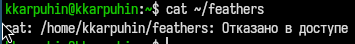
\includegraphics[width=0.6\linewidth,height=\textheight,keepaspectratio]{./image/33.png}

\textbf{4.9} Возврат права на чтение:

\begin{Shaded}
\begin{Highlighting}[]
\FunctionTok{chmod}\NormalTok{ u+r \textasciitilde{}/feathers}
\end{Highlighting}
\end{Shaded}
\end{frame}

\begin{frame}[fragile]{Права на выполнение для каталога}
\protect\phantomsection\label{ux43fux440ux430ux432ux430-ux43dux430-ux432ux44bux43fux43eux43bux43dux435ux43dux438ux435-ux434ux43bux44f-ux43aux430ux442ux430ux43bux43eux433ux430}
\textbf{4.10} Лишение владельца права на выполнение каталога
\texttt{\textasciitilde{}/play}:

\begin{Shaded}
\begin{Highlighting}[]
\FunctionTok{chmod}\NormalTok{ u{-}x \textasciitilde{}/play}
\end{Highlighting}
\end{Shaded}

\textbf{4.11} Попытка перехода (\texttt{cd\ \textasciitilde{}/play}) →
ошибка \texttt{Permission\ denied}. \textbf{4.12} Возврат права на
выполнение:

\begin{Shaded}
\begin{Highlighting}[]
\FunctionTok{chmod}\NormalTok{ u+x \textasciitilde{}/play}
\end{Highlighting}
\end{Shaded}
\end{frame}

\section{Системные
команды}\label{ux441ux438ux441ux442ux435ux43cux43dux44bux435-ux43aux43eux43cux430ux43dux434ux44b}

\begin{frame}[fragile]{mount, fsck, mkfs, kill}
\protect\phantomsection\label{mount-fsck-mkfs-kill}
{\def\LTcaptype{none} % do not increment counter
\begin{longtable}[]{@{}lll@{}}
\toprule\noalign{}
Команда & Назначение & Пример \\
\midrule\noalign{}
\endhead
\texttt{mount} & Монтирование файловых систем &
\texttt{mount\ /dev/sdb1\ /mnt} \\
\texttt{fsck} & Проверка и восстановление ФС &
\texttt{fsck\ /dev/sda1} \\
\texttt{mkfs} & Создание файловой системы &
\texttt{mkfs.ext4\ /dev/sdb1} \\
\texttt{kill} & Отправка сигналов процессам & \texttt{kill\ -9\ 1234} \\
\bottomrule\noalign{}
\end{longtable}
}

\begin{itemize}[<+->]
\tightlist
\item
  \texttt{man\ mount} --- справка по монтированию.
\item
  \texttt{man\ fsck} --- параметры проверки ФС.
\item
  \texttt{man\ mkfs} --- создание ФС разных типов.
\item
  \texttt{man\ kill} --- список сигналов (\texttt{-l}).
\end{itemize}
\end{frame}

\section{Контрольные вопросы
(1-7)}\label{ux43aux43eux43dux442ux440ux43eux43bux44cux43dux44bux435-ux432ux43eux43fux440ux43eux441ux44b-1-7}

\begin{frame}[fragile]{Контрольные вопросы (1-7)}
\begin{enumerate}[<+->]
\tightlist
\item
  \textbf{Командная строка} --- текстовый интерфейс взаимодействия с ОС.
\item
  \textbf{Абсолютный путь} текущего каталога: \texttt{pwd}.
\item
  \textbf{Тип файлов и их имена}: \texttt{ls\ -F}.
\item
  \textbf{Скрытые файлы}: \texttt{ls\ -a} или \texttt{ls\ -la}.
\item
  \textbf{Удаление файла}: \texttt{rm}, \textbf{пустого каталога}:
  \texttt{rmdir}. Можно одной командой: \texttt{rm\ -r}.
\item
  \textbf{История команд}: \texttt{history}.
\item
  \textbf{Модифицированное выполнение}: \texttt{!15} или
  \texttt{\^{}old\^{}new}.
\end{enumerate}
\end{frame}

\section{Контрольные вопросы
(8-13)}\label{ux43aux43eux43dux442ux440ux43eux43bux44cux43dux44bux435-ux432ux43eux43fux440ux43eux441ux44b-8-13}

\begin{frame}[fragile]{Контрольные вопросы (8-13)}
\begin{enumerate}[<+->]
\setcounter{enumi}{7}
\tightlist
\item
  \textbf{Несколько команд в одной строке}: \texttt{;}, \texttt{\&\&},
  \texttt{\textbar{}\textbar{}}. Пример: \texttt{cd\ /tmp;\ ls}.
\item
  \textbf{Экранирование}: \texttt{\textbackslash{}}. Пример:
  \texttt{echo\ Hello\textbackslash{}\ world}.
\item
  \textbf{\texttt{ls\ -l}}: права, ссылки, владелец, группа, размер,
  дата, имя.
\item
  \textbf{Относительный путь}: \texttt{documents}, \textbf{абсолютный}:
  \texttt{/home/user/documents}.
\item
  \textbf{Справка}: \texttt{man\ \textless{}команда\textgreater{}} или
  \texttt{\textless{}команда\textgreater{}\ -\/-help}.
\item
  \textbf{Автодополнение}: \texttt{Tab}.
\end{enumerate}
\end{frame}

\section{Выводы}\label{ux432ux44bux432ux43eux434ux44b}

\begin{frame}[fragile]{Результаты работы}
\protect\phantomsection\label{ux440ux435ux437ux443ux43bux44cux442ux430ux442ux44b-ux440ux430ux431ux43eux442ux44b}
\begin{itemize}[<+->]
\tightlist
\item
  Освоил работу с Midnight Commander (mc): навигация, функциональные
  клавиши, панели, поиск, редактирование.
\item
  Приобрел практические навыки работы с командами \texttt{cp},
  \texttt{mv}, \texttt{chmod}.
\item
  Изучил механизм изменения прав доступа к файлам и каталогам.
\item
  Познакомился с системными командами \texttt{mount}, \texttt{fsck},
  \texttt{mkfs}, \texttt{kill}.
\item
  Научился создавать псевдонимы в \texttt{.bashrc} для ускорения работы.
\end{itemize}
\end{frame}

\begin{frame}[fragile]{Ключевые навыки}
\protect\phantomsection\label{ux43aux43bux44eux447ux435ux432ux44bux435-ux43dux430ux432ux44bux43aux438}
\begin{itemize}[<+->]
\tightlist
\item
  Уверенная навигация по файловой системе Linux.
\item
  Копирование, перемещение, переименование файлов и каталогов.
\item
  Управление правами доступа.
\item
  Использование справочной системы \texttt{man}.
\item
  Работа с историей команд.
\end{itemize}
\end{frame}

\section{Список
литературы}\label{ux441ux43fux438ux441ux43eux43a-ux43bux438ux442ux435ux440ux430ux442ux443ux440ux44b}

\begin{frame}{Список литературы}
\protect\phantomsection\label{refs}
\end{frame}




\end{document}
